\documentclass[a4paper,12pt]{article} % This defines the style of your paper

\usepackage[top = 2.5cm, bottom = 2.5cm, left = 2.5cm, right = 2.5cm]{geometry} 

\usepackage[utf8]{inputenc}
\usepackage[english]{babel}

\usepackage{multirow} % Multi-row is for tables with multiple rows within one cell.
\usepackage{booktabs} % For even nicer tables.

\usepackage{graphicx}
\usepackage{amsmath}
\usepackage{amsfonts}
\usepackage{listings}

\usepackage{setspace}

\usepackage{float}

\usepackage{fancyhdr}


\pagestyle{fancy}

\fancyhf{}

\rhead{\footnotesize Jiří Klepl}

\cfoot{\footnotesize \thepage} 

\begin{document}

\thispagestyle{empty}

\begin{center}
    {\Large \bf Simultaneous contrast}
    \vspace{2mm}

    {\bf Jiří Klepl}
\end{center}

\section{What is simultaneous contrast}

Simultaneous contrast is an effect which happens when a subject is exposed to two objects of the similar color in a different spatial context simultaneously, the one surrounded by lighter obstacles will appear darker than it actually is. It is one of the most common optical illusions probably caused by how the brain is conditioned to see brightness and color differences (Weber's law, or evolution? It is not really clear).

Figure \ref{experiment_png} shows a single test of the experiment, the small square patch positioned on the light square appears darker then if it was compared to square patch positioned freely on the black background without any surroundings.

The popular illusion is usually setup in a way that the two square patches are of the exactly same color. This experiment, however, attempts to find the brightness (measured by ``rgb luminance'') of the right square patch which is subjectively equal to the one on the left.

\begin{figure}[htb!]
    \centering
    \caption{Experiment example}
    \label{experiment_png}
    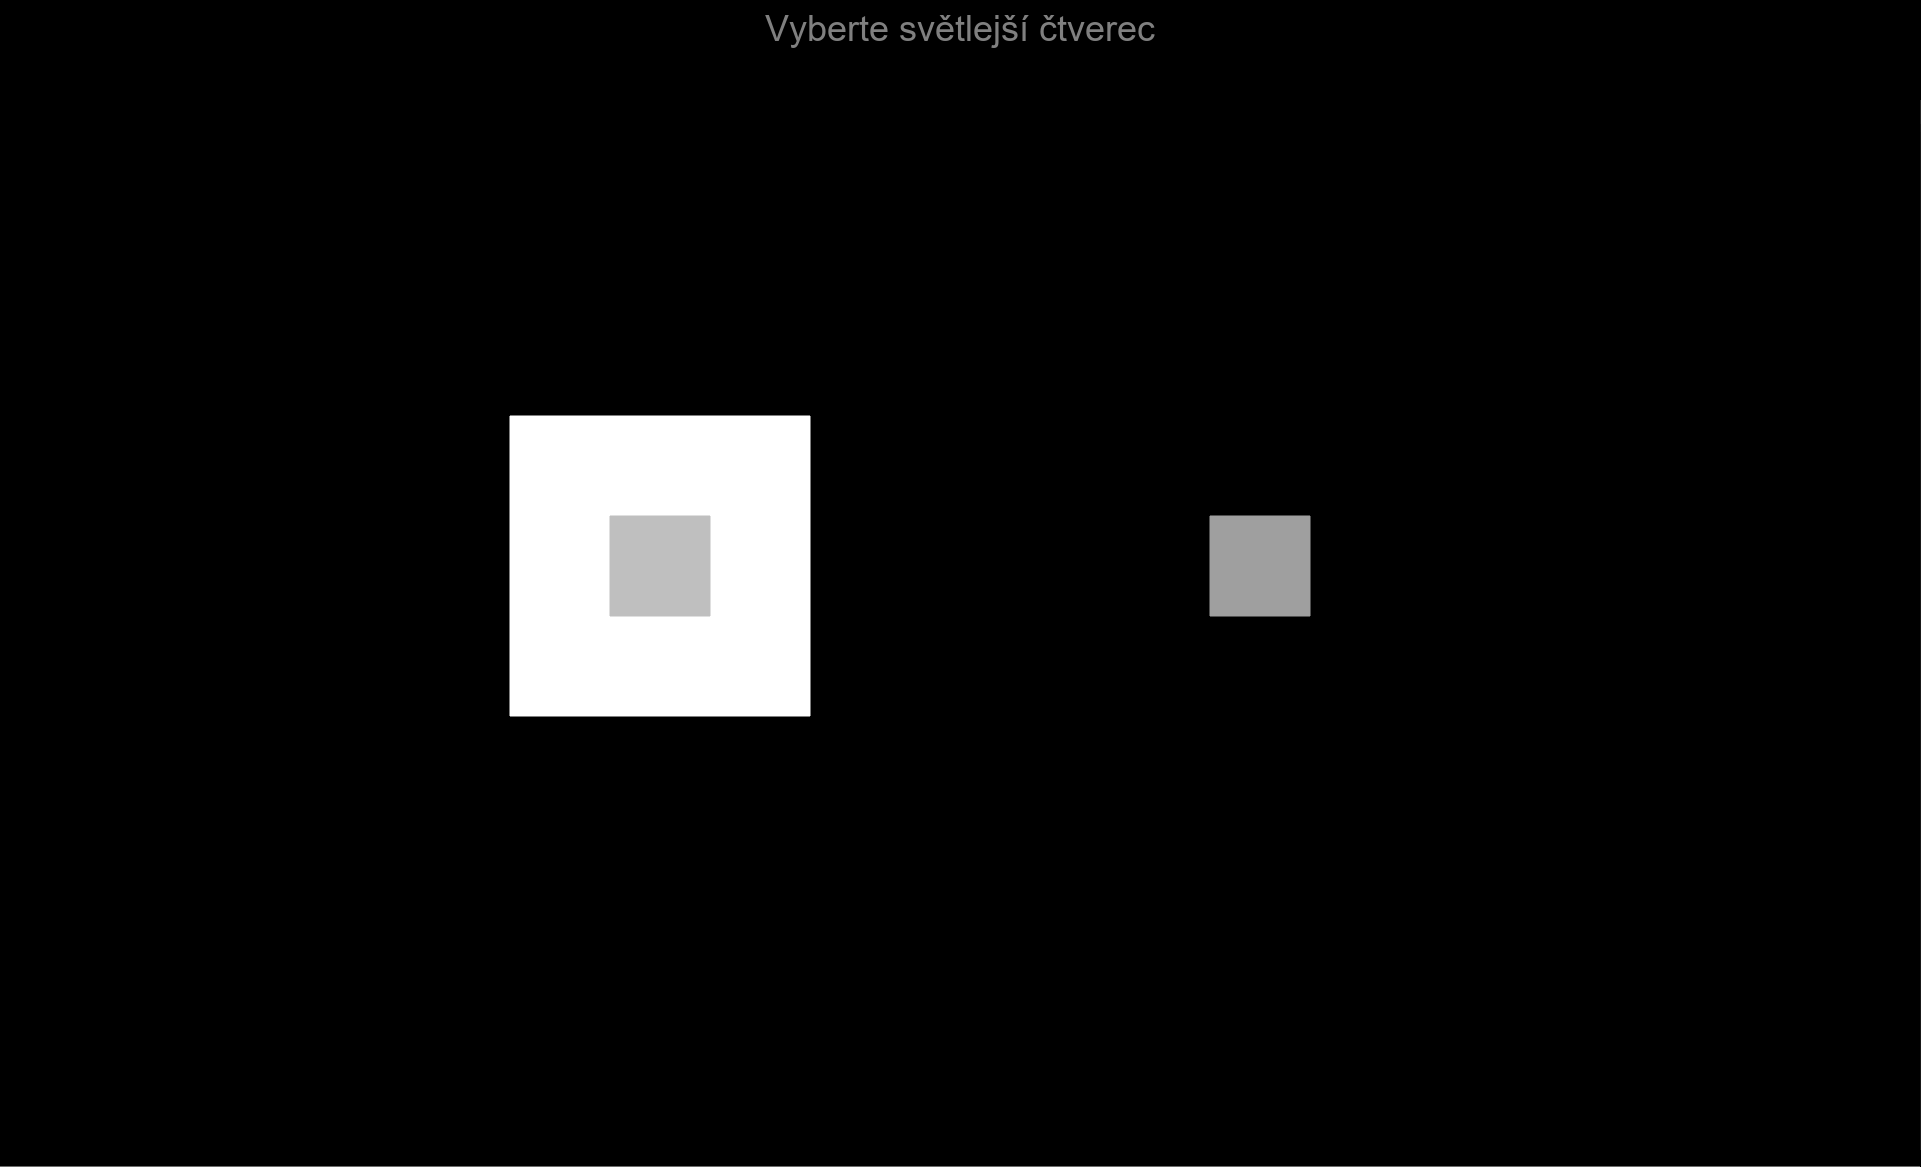
\includegraphics[width=\linewidth]{experiment.png}
\end{figure}

\section{Experiment setup}

The experiment consists of two sets of contrast tests (both having 9 possible values each replicated 30 times), one is in gray monochrome, the other in green - choice of this particular color was inspired by the fact human eye is most sensitive in this color spectrum. Our hypothesis was that the luminance of the test patch subjectively equal to the left patch would be slightly below $.5$ (the luminance value of the left patch).

The green version was adjusted by changing all other colors' luminance levels to minimum.

The computer on which the experiment was run has a 24'' monitor with the resolution of 1920 x 1200. It was set in a room lit by a regular dimmed LED lightbulb.

The colors used for the experiment were picked from the interval 5:13 for both the black-and-white version and the green version (this reflects the hypothesis by setting the expected result in the middle of the measured interval).

It was ensured the participants knew what was expected of them. They all had undergone the suggested training pre-run and then the two experiments in the suggested order with a short break in-between.

\section{Analysis}

For the analysis, all participants were given numeric names to anonymize them. This is the only physical manipulation done to the files generated by the PsychoPy software.

The confidence interval probability for the threshold value of luminance was set to $95\%$, as is the standard generally used in statistics.

\section{Results}

We use the \lstinline{quickpsy} function to fit the psychometric function with the explanatory value being \lstinline{rgb_luminance} and the response variable the number representing the choice of the lighter patch as dictated by the assignment ($0$ for the left one, $1$ for the (test) right one).

\subsection{Thresholds table}

The table \ref{thresholds_table} (generated by the \lstinline{xtable} function) shows resulting thresholds for subjective luminance equivalence of the patches in the experiment for each participant, lower session numbers with the same participant number show the gray version of the experiment, higher session numbers then show the green version.

\lstinline{threshold} shows the mean value, \lstinline{threshold_inf} and \lstinline{threshold_sup} then show the lower and higher bounds (respectively) for the $95\%$ confidence interval.

% latex table generated in R 4.0.3 by xtable 1.8-4 package
% Fri Jan 22 14:14:28 2021
\begin{table}[!htb]
    \centering
    \caption{Thresholds table}
    \label{thresholds_table}
    \begin{tabular}{rrrrrr}
      \hline
     & participant & session & threshold & threshold\_inf & threshold\_sup \\ 
      \hline
    1 & 1.00 & 2.00 & 0.31 & 0.29 & 0.33 \\ 
      2 & 1.00 & 3.00 & 0.27 & 0.25 & 0.28 \\ 
      3 & 2.00 & 10.00 & 0.33 & 0.31 & 0.35 \\ 
      4 & 2.00 & 12.00 & 0.35 & 0.33 & 0.37 \\ 
      5 & 3.00 & 6.00 & 0.29 & 0.25 & 0.31 \\ 
      6 & 3.00 & 7.00 & 0.23 & 0.18 & 0.28 \\ 
       \hline
    \end{tabular}
\end{table}

\pagebreak

\subsection{Interesting plots}

The figures \ref{figure_002} and \ref{figure_003} show very interesting results: almost everyone performed slightly worse on the green version of the experiment, with an exception of participant 002 who performed a little bit better. Participant 003 performed much worse on the colored version and their results were outside of the measured interval.

\begin{figure}[!htb]
    \centering
    \caption{Participant 002 - the gray \& green version (sessions 010 and 012)}
    \label{figure_002}
    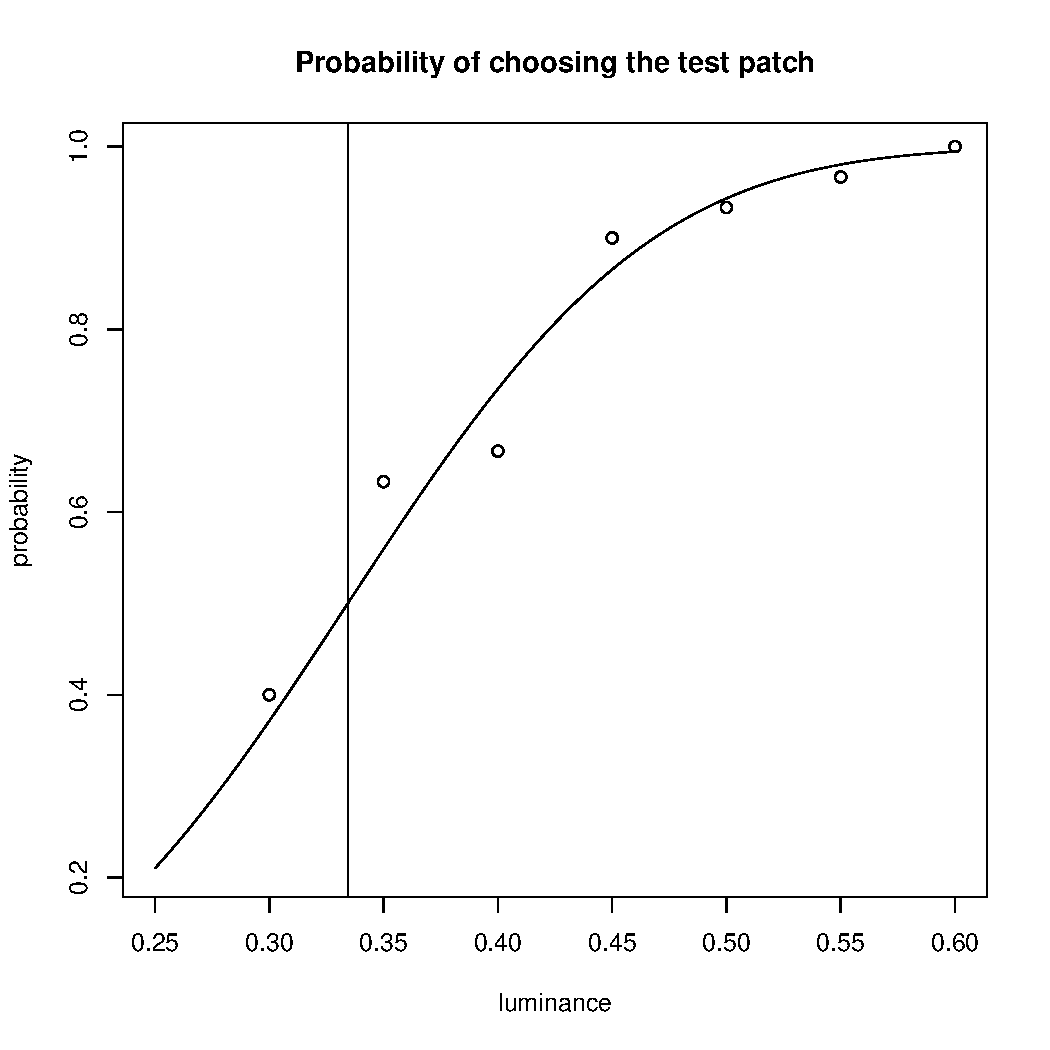
\includegraphics[width=3in]{2-10-plot.pdf}
    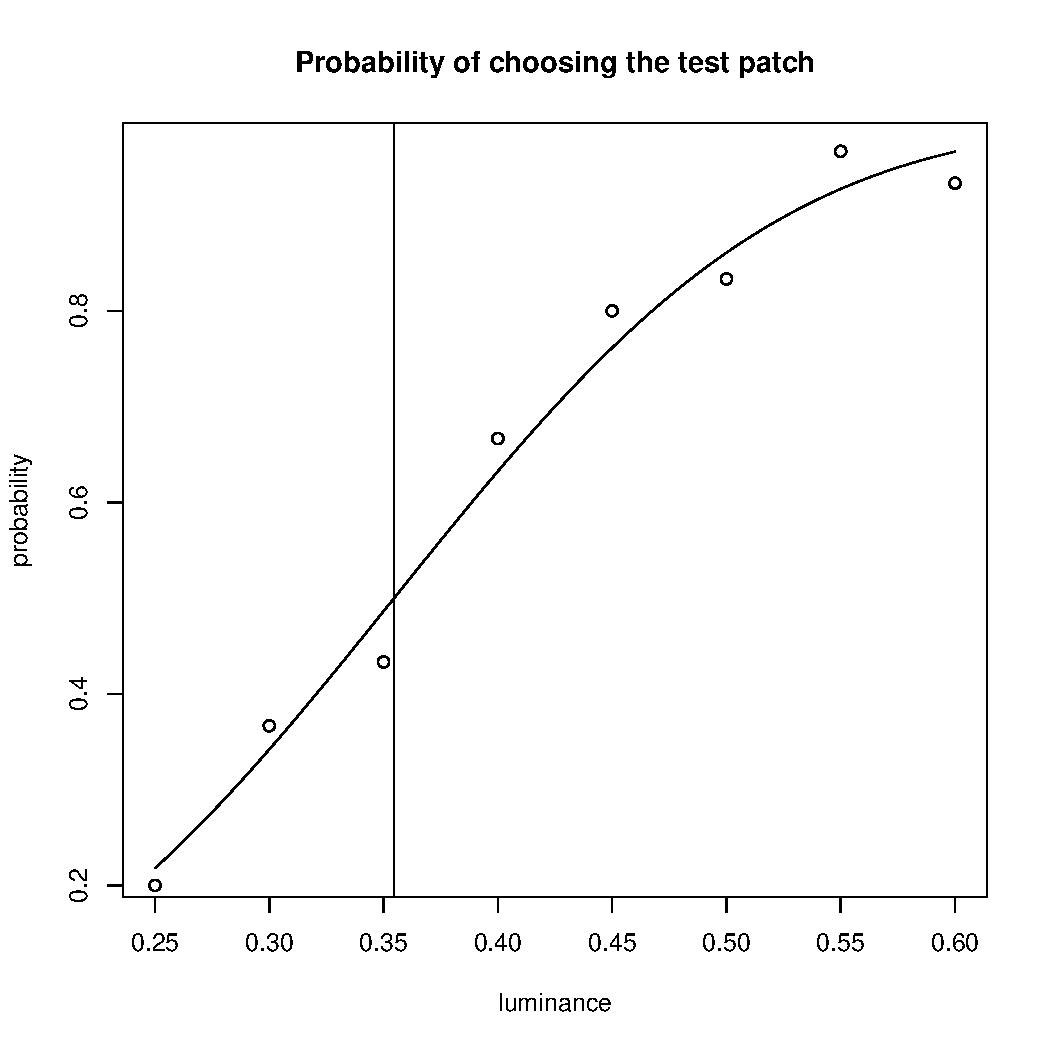
\includegraphics[width=3in]{2-12-plot.pdf}
\end{figure}

\begin{figure}[!htb]
    \centering
    \caption{Participant 003 - the green version (session 007)}
    \label{figure_003}
    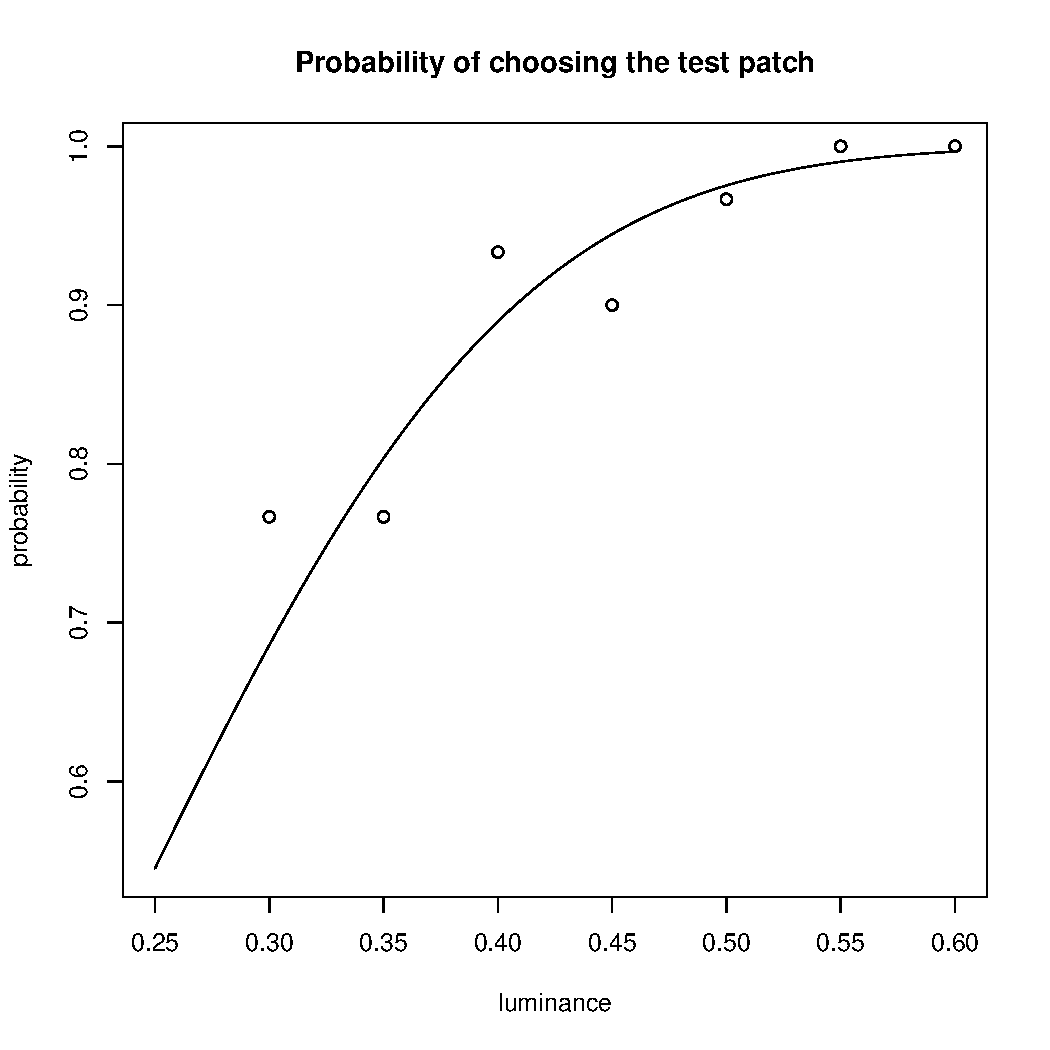
\includegraphics[width=4in]{3-7-plot.pdf}
\end{figure}

\pagebreak

\section{Conclusion}

We can conclude that the effect of simultaneous contrast makes the subjectively equal test patch be the one with luminance of approximately $.3$ (color luminance in the green test), compared to the true value of $.5$.

The fact that the subjectively equal test patch is darker than the left one is not really surprising (eg. aforementioned Weber's law), but the extent of this effect is. The even more surprising bit is that this value appeared to be consistent regardless of the subjects' knowledge of the setup of the experiment, their state and their attention given for the experiment.

One more interesting thing is the psychometric curve seems to be cut-off at the bottom part (as the psychometric curve should start at $0$). This is due to our underestimating of the simultaneous contrast's effect prior to the experiment.

The results didn't show any consistent difference between the gray and the green version, the sample size is too small to draw any conclusions from that.

If we were to perform further research on this we should watch more parameters and increase the sample size.

\end{document}
